HackstadtHackstadt%!TEX root = ../Thesis.tex
\chapter{Linking brain-wide gene expression and neuroimaging data}
\label{ch:Chapter4}
\fancyhead[R]{\textit{Chapter.} \textit{\thechapter: }\textit{Linking brain-wide gene expression and neuroimaging data}}


% Insert author names, affiliations and corresponding author email (do not include titles, positions, or degrees).

\textbf{Aurina Arnatkevi\u{c}i\={u}t\.{e}},
Ben D. Fulcher,
Alex Fornito (2019).
A practical guide to linking brain-wide gene expression and neuroimaging data. Published in \textit{
NeuroImage}.\\
DOI: \url{https://doi.org/10.1016/j.neuroimage.2019.01.011} % Please use "sentence case" for title and headings (capitalize only the first word in a title (or heading), the first word in a subtitle (or subheading), and any proper nouns).
Supplementary materials can be found in Appendix B.


\section*{Preamble}
Preamble text.

\newpage

\section*{Abstract}
The recent availability of comprehensive, brain-wide gene expression atlases such as the Allen Human Brain Atlas (AHBA) has opened new opportunities for understanding how spatial variations on the molecular scale relate to the macroscopic neuroimaging phenotypes. A rapidly growing body of literature is demonstrating relationships between gene expression and diverse properties of brain structure and function, but approaches for combining expression atlas data with neuroimaging are highly inconsistent, with substantial variations in how the expression data are processed. The degree to which these methodological variations affect findings is unclear. Here, we outline a seven-step analysis pipeline for relating brain-wide transcriptomic and neuroimaging data and compare how different processing choices influence the resulting data. We suggest that studies using AHBA should work towards a unified data processing pipeline to ensure consistent and reproducible results in this burgeoning field.

\section{Introduction}

Over the past two decades, human imaging genetics has emerged as a powerful strategy for understanding the molecular basis of macroscopic neural phenotypes measured across the entire brain \citep{Meyer-Lindenberg2006a,Munoz2009,Arslan2015,Hashimoto2015}. Traditionally, this work has involved correlating allelic variation at one or more genetic loci with variation in one or more imaging-derived phenotypes (IDPs), initially through candidate gene studies and more recently at a genome-wide level. The latter has been facilitated by the formation of large consortia, such as ENIGMA \citep{Thompson2014}. A common assumption in this work is that variants associated with an IDP (or nearby variants tagged by the associated variant) influence gene expression or protein abundance, which in turn alters cellular function and ultimately affects the studied IDP. However, multiple environmental and other factors can impact gene activity \citep{Fraser2005,Choi2007,Cole2009} and the functional roles of many IDP-linked variants, which are usually identified through large-scale statistical analyses, are often unknown. As a result, the mechanisms through which a given variant may influence phenotypic variation can be unclear. Moreover, the expression levels of many genes vary substantially across brain regions \citep{Hawrylycz2015}, and these spatial variations cannot be inferred from DNA sequence alone.

Assays of gene expression provide a more direct measure of gene function. Expression assays are invasive, requiring direct access to neural tissue, and technical limitations have historically constrained analyses of gene expression in the brain to small sets of areas studied in isolation. Recent advances in the development of high-throughput tissue processing and bioinformatics pipelines have overcome these limitations, resulting in datasets of gene expression across a large fraction of the genome in a large number of brain regions, and through various stages of development [see \citet{Keil2018} for a detailed overview]. While some of the human atlases span multiple brain areas, only the Allen Human Brain Atlas (AHBA) offers high resolution coverage of nearly the entire brain, comprising expression measures for more than \num{20000} genes taken from \num{3702} spatially distinct tissue samples. Critically, the samples have been mapped into the stereotaxic space, allowing researchers to directly relate spatial variations in gene expression to spatial variations in IDPs (for more details on the AHBA see \ref{app:AppendixCh4_1}).

This unprecedented capacity to link molecular function to macroscale brain organization has given rise to the nascent field of imaging transcriptomics [for an overview, see \citep{Fornito2019}], which has begun to yield new insights into how regional variations in gene expression relate to: functional connectivity within canonical resting-state networks \citep{Richiardi2015,Forest2017};
fiber tract connectivity between brain regions \citep{Goel2014};
temporal and topological properties of large-scale brain functional networks \citep{Cioli2014b,Vertes2016b};
the specialization of cortical and subcrotical areas \citep{Krienen2016,Parkes2017,Anderson2018};
regional maturation during embryonic and adolescent brain development \citep{Kirsch2016a,Whitaker2016a};
and pathological changes in brain disorders \citep{Rittman2016,Romme2017,McColgan2018,Romero-Garcia2018a}. Software toolboxes to facilitate the integration of brain-wide transcriptomic and imaging data have also been developed \citep{French2015,Gorgolewski2015,Rizzo2016,Rittman2017}.

Unlike behavioral genetics or studies of structural DNA variants, where the goal is to understand how genetic variation correlates with phenotypic variability across a sample of individuals, analyses in imaging transcriptomics are concerned with identifying spatial correlations between gene expression patterns and some property of brain structure or function \citep{Fornito2019}. In other words, the goal is to identify genes with spatial profiles of expression that track anatomical variations in a given IDP. These analyses are often highly multivariate, involving expression measures of around \num{20000} genes in each of around $10^{2}–10^{3}$ brain regions, being related to one or more distinct IDPs quantified in each region. This complexity is compounded by the fact that both imaging data and gene expression data undergo extensive processing prior to analysis.

The impact of data processing choices on the results of neuroimaging analyses is well documented, with strategies for the correction of motion-related and global signal fluctuations in functional MRI being a prime example \citep{Power2015a,Power2017,Ciric2017,Parkes2018}. Comparable scrutiny has not yet been applied to the many processing choices that can affect the analysis of transcriptomic atlases and their relation to IDPs. At the time of writing, more than $30$ studies have linked the AHBA gene expression measures to human neuroimaging data. The lack of a standard processing pipeline for gene expression data means that the degree to which the results of this work are robust to different methodological choices remains unclear.

As the field develops, it is important to establish methodological guidelines to ensure consistent and reproducible results, and to support valid interpretation. In this paper, we offer a practical guide to some of the key steps in processing the AHBA gene expression data and examine the potential impact of methodological choices available at each step. We focus on the AHBA, as it is the most spatially comprehensive and widely used gene expression atlas in the field \citep{Hawrylycz2012}.

The paper is organised as follows. We begin by summarizing some basic aspects of how gene expression is quantified, and general characteristics of the AHBA. We then outline several key steps in a basic workflow for relating gene expression measures to imaging data and examine the impact of methodological choices at each step. In the final section, we make some recommendations for best practice and provide directions for further research.


\section{Measuring gene expression}

Gene expression is a process through which genetic information encoded by sequences of DNA is read and used to synthesize a particular gene product, such as a protein or RNA molecule \citep{Szymanski2002}. The order of amino acids within each gene determines the structure and function of the resulting product, which in turn affects cellular function and drives phenotypic variability. While the DNA sequence of each cell in the organism is identical, different cells and anatomical structures express different phenotypes (e.g., neurons versus lymphocytes) due to differences in gene expression. The process through which a sequence of DNA is expressed is complex, but (for present purposes) can be divided into two main stages: (1) transcription, which occurs when an unwound segment of DNA is read to produce messenger RNA (mRNA); and (2) translation, which occurs when mRNA is used to synthesize proteins \citep{Krebs2014}. Gene expression is commonly approximated by measuring mRNA levels of a particular gene and is thus an index of gene transcriptional activity. Gene transcription is an indirect proxy for protein abundance, which is ultimately determined by gene translation. This distinction is important as several studies have shown that mRNA and protein levels within a tissue can vary significantly \citep{Futcher1999,Gygi1999,Greenbaum2003}, and gene expression (transcriptional activity) and protein abundance (translational activity) are not always positively correlated \citep{Margineantu2007,Schwanhausser2011}.

In the AHBA, transcriptional activity has been measured using microarray, which quantifies the expression levels of thousands of genes at once by measuring the hybridization of cRNA (Cy3-labeled RNA) in a tissue sample to a  particular spot on the microarray chip. Each of these spots, called probes, maps to a unique location of the DNA and contains single-stranded nucleic acid profiles that are ready to anneal to their complementary targets in the process of hybridization. Relative levels of gene expression in a tissue sample are then quantified by measuring the fluorescence at each sequence-specific location, which is proportional to the amount of cRNA in a sample \citep{Tarca2006}. This method provides a cost-effective way to measure gene expression in high-throughput manner. However, it is limited to known gene sequences, is prone to background noise due to indirect assessment of expression values, and spatial biases can result from variability in the lateral diffusion of target molecules on the chip \citep{Steger2011}. Expression measures can also be affected by cross-hybridization artefacts arising when cRNA anneals to an imperfectly matched probe.

Microarray is typically performed on bulk tissue samples, and the cellular composition of a sample can strongly influence its gene expression profile. As a result, two samples with varying densities of different cell types may show transcriptional differences simply because of their different cellular composition. This is an important consideration when comparing data acquired from samples taken from different parts of the brain, since variations in the density of distinct cell types may drive differences in regional gene expression. In addition, variations in the way tissue samples are acquired, handled and processed, age at death \citep{Glass2013}, sex \citep{Berchtold2008,Trabzuni2013}, ethnicity \citep{Spielman2007}, brain pH \citep{Mexal2006}, post-mortem interval \citep{Zhu2017}, and RNA degradation \citep{Jaksik2015}, can all affect expression measures. Another potential influence arises from batch effects, caused by samples being processed at different times, by different staff, or in different labs; even changing atmospheric ozone levels can impact the final measures \citep{Fare2003} [see \citet{Scherer2009} for an overview]. The Allen Institute has implemented a series of steps to mitigate this variability as much as possible, as outlined in Allen Human Brain Atlas technical white paper \citep{AHBAdoc}.

One final consideration is that any individual gene expression assay provides a static snapshot of a dynamic process. Gene expression changes through development, and as a function of experience, environmental exposures and other factors \citep{Fraser2005,Choi2007,Berchtold2008,Cole2009,Birdsill2011,Naumova2012,Kumar2013}.
The further advancement of developmental atlases of gene expression \citep{Johnson2009,Colantuoni2011,Kang2011,Fertuzinhos2014,Bakken2016} will help to shed light on these dynamic processes.

% METHODS: connectivity data
\section{A general workflow for processing brain-wide transcriptomic data}
The AHBA consists of microarray data in \num{3702} spatially distinct samples taken from six neurotypical adult brains. The samples are distributed across cortical, subcortical, brainstem and cerebellar regions in each brain, and quantify the expression levels of more than \num{20000} genes (for more details see \ref{app:AppendixCh4_1}). Different brain regions were sampled across each of the six AHBA donors to maximize spatial coverage. Figure \ref{fig:Ch4Fig1} shows the  variability of coverage across individual brains.

Each tissue sample is associated with a numeric structure ID, name and structure label (cortex, cerebellum, or brainstem) in addition to the MRI voxel coordinates in native image space and MNI stereotaxic coordinates, which can be used to match samples to other imaging data (Figure \ref{fig:Ch4Fig1}). The AHBA also provides: (1) a binary indicator of when the level of a given transcript exceeds background levels, which can be used for quality control purposes; (2) RNA-seq data for a subset of tissue samples in two donor brains ($120$ samples each), which can be used for cross-validating expression measures (as we show below); and (3) magnetic resonance images, including T1-weighted, T2-weighted, T2-weighted gradient echo and FLAIR scans for all six brains, and diffusion-weighted images for two brains. These scans were collected prior to the dissection for anatomical visualization.

\begin{figure}[h!]
  \centering
    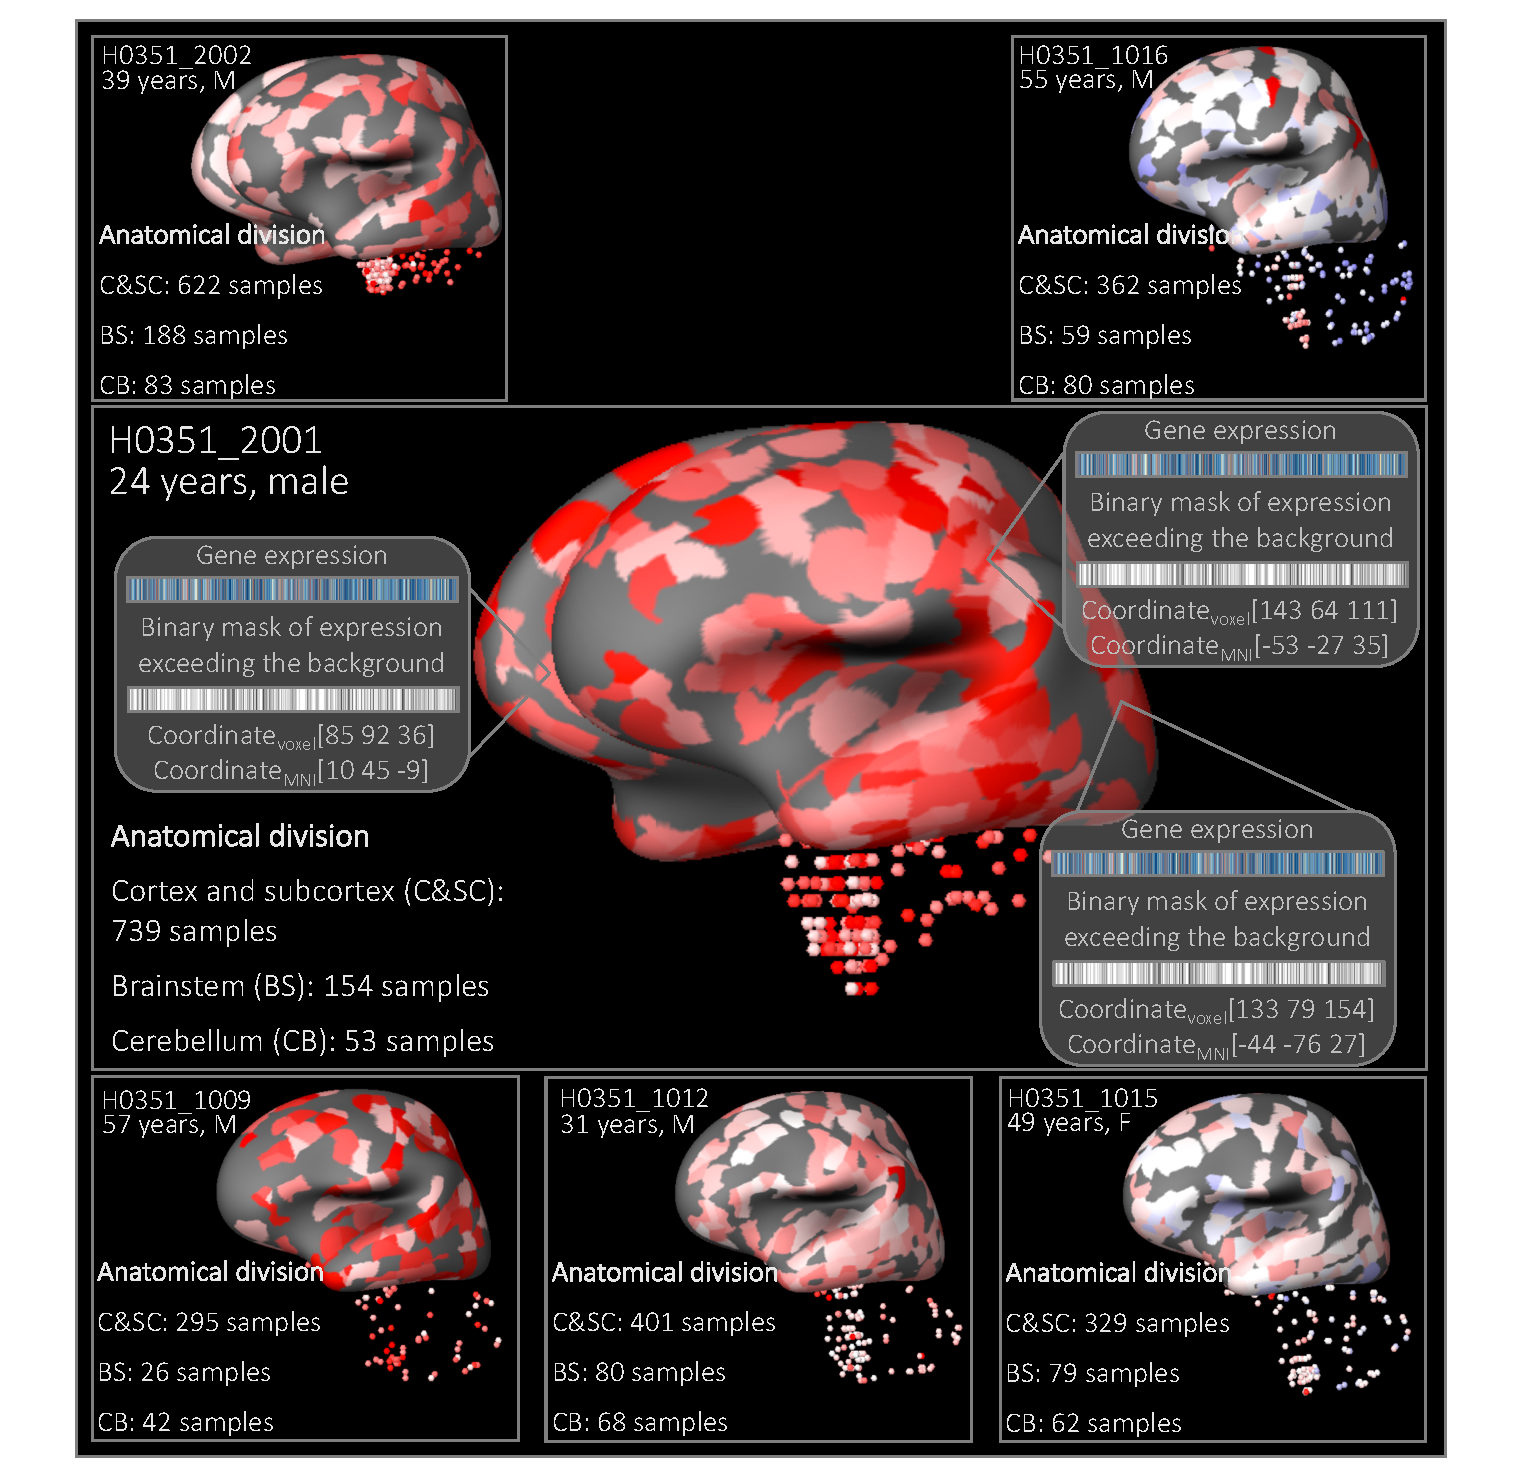
\includegraphics[width=1\textwidth]{Chapter4/Ch4Fig1.pdf}
\caption{\textbf{A schematic representation of expression data for a selected representative gene: CLRN1}. Discrete tissue samples in each brain are represented as colored areas on a grey brain surface. Color corresponds to the gene expression level of each sample relative to all other samples combined over all six brains ($z$-score): red (high), blue (low). The size of the patch is not representative of the size of the actual tissue sample used to quantify gene expression (which was much smaller than shown). The patch has been padded out by the AHBA online platform as a visual aid. The number of samples in each anatomical division: cortex and subcortex (C\&SC), brainstem (BS) and cerebellum (CB) for every donor brain is listed. Middle: A schematic representation of available data for each sample which includes expression values for $\sim$\num{20000} genes, a binary indication of whether the expression levels exceed background noise, and native voxel and MNI coordinates for each sample. Brain representation produced using Brain Explorer 2 (2006-2015 Allen Institute for Brain Science; available from: \url{http://human.brain-map.org/static/brainexplorer}). }
\label{fig:Ch4Fig1}
\end{figure}

The AHBA samples were processed over approximately three years, which raises concerns about possible batch effects. Expression data were subjected to normalization procedures within a single brain, as well as between brains, to minimize the effect of non-biological biases such as array-specific differences, dissection method, and RNA quality differences among others, while maintaining biologically-relevant variance. Detailed information about the normalization is provided in the technical white paper \citep{AHBAdoc}. Despite these procedures, we show below that large inter-individual differences in gene expression remain, such that samples from the same brain tend to have more similar gene expression compared to the samples from other brains. These differences must be taken into account when combining data across all six brains.

Beyond the processing steps applied by the Allen Institute, a number of other procedures are required to link expression measures and neuroimaging data. Here we outline seven major steps, summarized in Figure \ref{fig:Ch4Fig2}, which represent the core features of a typical workflow:
(i) verifying probe-to-gene annotations;
(ii) filtering of probes that do not exceed background noise;
(iii) probe selection, where representative probes (or a summary measure) are selected to index expression for a gene;
(iv) sample assignment, where tissue samples from the AHBA are mapped to specific brain regions in an imaging dataset;
(v) normalization of expression measures to account for inter-individual differences and outlying values;
(vi) gene-set filtering, to remove genes that are inconsistently expressed across six brains and/or to select genes in a hypothesis-driven way based on the research question.
(vii) accounting for the spatial patterns in gene expression;

The first six processing steps produce the region $\times$ gene matrix that can be used for the regional analyses.
The final step of accounting for the autocorrelation in the gene expression measures depends on the particular research question.
The potential need to account for spatial effects arises because gene expression is more strongly correlated between samples that are separated by short distances compared to those that are far apart, a pattern that has been described in humans
\citep{Richiardi2015,Krienen2016,Vertes2016b,Pantazatos2017}, mouse \citep{Fulcher2016} and \textit{C.elegans} \citep{Arnatkeviciute2018}.
Although this spatial autocorrelation is, in itself, an important neurobiological feature of the brain transcriptome \citep{Gryglewski2018, Fornito2019},
it is critical for any analysis claiming a specific association between spatial variations in gene expression and a given IDP to show that the association is not attributable to lower-order spatial gradients of gene expression.

In the following sections, we outline some of the choices that can be made at each of these steps and consider their impact on analysis with some recommendations summarized in the conclusions section. Code and data are available at github \url{https://github.com/BMHLab/AHBAprocessing} and figshare \url{https://doi.org/10.6084/m9.figshare.6852911} respectively.

\begin{figure}[h!]
  \centering
    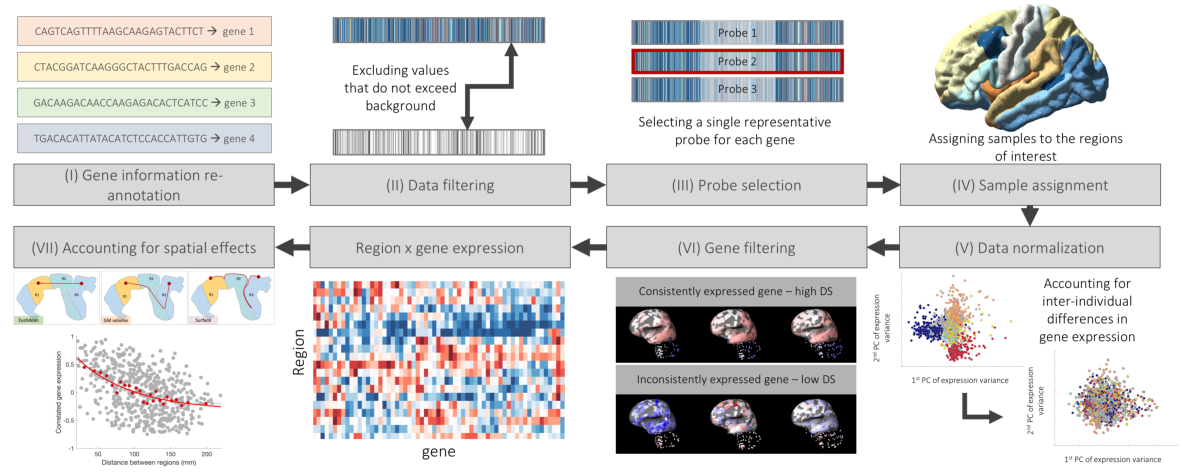
\includegraphics[width=1\textwidth]{Chapter4/Ch4Fig2.pdf}
\caption{\textbf{Schematic of a general workflow for combining AHBA and neuroimaging data.} The basic workflow involves: (i) confirming and updating probe-to-gene annotations using the latest available data; (ii) data filtering, where expression values that do not exceed background are removed; (iii) probe selection, which, for genes indexed by multiple probes, involves selecting a single representative measure to represent the expression of that gene across all donor brains; (iv) sample assignment, where tissue samples from the AHBA are mapped to specific brain regions in an imaging dataset; (v) normalization of expression measures to account for inter-individual differences and outlying values; (vi) gene-set filtering, to remove genes that are inconsistently expressed across six brains and/or to select genes in a hypothesis-driven way [here we show a gene with consistent expression across three individual brains in the top row and a gene with low consistency in the bottom row, where consistency is measured using a metric called differential stability, or DS \citep{Hawrylycz2015}]. The application of these six steps results in a region $\times$ gene expression data matrix that can be further used for the analysis. An important consideration for analyses involving transcriptional data is (vii) accounting for spatial effects.}

\label{fig:Ch4Fig2}
\end{figure}

\subsection{Step 1. Probe-to-gene re-annotation}

In microarray experiments, probe sequences correspond to a unique portion of DNA and are assigned to genes based on available genome sequencing databases \citep{OLeary2016}. While the AHBA (and other platforms) provide annotation tables where probes are mapped to genes, this information gets outdated with each update of the sequencing databases. An accurate probe-to-gene mapping is essential for obtaining  biologically meaningful findings. It is therefore necessary to re-assign probes to genes using the most current information available. This re-annotation can be done using several methods and toolboxes, some of which are summarized in Table \ref{Table1}. To our knowledge, only three studies using the AHBA have performed probe-to-gene re-annotation \citep{Richiardi2015,Eising2016,Romero-Garcia2018}.

\begin{table}[h!]
\caption{Tools that can be used to update probe-to-gene assignment.}
\label{Table1}
\resizebox{\textwidth}{!}{%
\begin{tabular}{ll}
\hline
\multicolumn{1}{c}{\textbf{Software}} & \multicolumn{1}{c}{\textbf{Description}} \\ \hline
Re-annotator & \begin{tabular}[c]{@{}l@{}}Command-line based re-annotation pipeline which uses probe sequence and mRNA reference database information \\ to identify genes that match specific microarray probe sequences. Can work with any type of probe sequence \\ data$^{a}$ but requires additional software tools (PERL, BWA, SAMtools, Annovar) and external data sources such as \\ a reference genome sequence and gene locations.\end{tabular} \\ \hline
BioMart & \begin{tabular}[c]{@{}l@{}}Web-based data mining tool that provides an easy way to employ the latest available information contained\\ in the Ensembl genome database - a comprehensive source of stable automatic annotation of the human genome \\ sequence. Limited to standard microarray platforms and cannot annotate custom probes in AHBA.\end{tabular} \\ \hline
AnnotationDbi & \begin{tabular}[c]{@{}l@{}}R-based software package in ‘Bioconductor’ providing a user interface and database connection code for\\ annotation data package. Limited to standard microarray platforms and cannot annotate custom probes in AHBA.\end{tabular} \\ \hline
\end{tabular}}
\begin{tablenotes}
     \item[1] $^{a}$ The probe sequence information that is needed to perform annotation using the Re-annotator pipeline can be accessed using the Allen Institute’s website application programming interface (API) (see \ref{app:AppendixCh4_7}) and is available at \url{https://doi.org/10.6084/m9.figshare.6852911}. Agilent probe sequences can also be downloaded  through the manufacturer's website (\url{https://earray.chem.agilent.com/earray/})
   \end{tablenotes}
\end{table}

To investigate how probe-to-gene annotations change over time, we supplied a list of all available $60$\,bp length AHBA probe sequences ($n =$ \num{58692}) to the Re-annotator toolkit \citep{Arloth2015} (Table \ref{Table1}). We found that \num{45821} probes ($78\%$) were uniquely annotated to a gene and could be related to an entrez ID - a stable identifier for a gene generated by the Entrez Gene database at the National Center for Biotechnology Information (NCBI). A total of $19\%$ of probes were not mapped to a gene, and just under $3\%$ were mapped to multiple genes and could not be unambiguously annotated. Of the probes that were unambiguously annotated to a gene, \num{3438} ($7.5\%$) of the annotations differed from those provided by the AHBA: \num{1287} probes were re-annotated to new genes and \num{2151} probes that were not previously assigned to any gene in the AHBA could now be annotated. Additionally, \num{6211} ($\sim10\%$) probes in the initial AHBA dataset had an inconsistent gene symbol, ID or gene name information according to the NCBI database (\url{https://www.ncbi.nlm.nih.gov/}), as of 5th March 2018. Because of these differences, we recommend obtaining probe-to-gene annotations and retrieving the gene symbol ID and name from the latest version of NCBI (\url{ftp://ftp.ncbi.nlm.nih.gov/gene/DATA/GENE_INFO/Mammalia/}). Hereafter, we present all analyses using this newly re-annotated set of \num{45821} probes, corresponding to \num{20232} unique genes.

\subsection{Step 2. Data filtering}

Microarray experiments are prone to background noise due to non-specific hybridization, so appropriate controls must be employed to discriminate expression signal from noise. Variability in measured intensity values is greater for lower hybridization intensities, where signal levels approach background \citep{Quackenbush2002a}. This problem is often addressed by removing a fixed percentage of probes with lowest intensity or using only array elements that show statistically significant expression differences (increase) from the background \citep{Quackenbush2002a}. Each probe in each sample of the AHBA has been assigned a binary indicator for whether it measures an expression signal that exceeds background levels, as defined using a t-test based criterion described in the AHBA white paper [\citep{AHBAdoc}, see Figure \ref{Fig1}]. Filtering genes using the AHBA binary indicator [intensity based filtering (IBF)] can have a marked effect on the final set of genes included for analysis, however only a few published studies using the AHBA data have reported using IBF \citep{Hawrylycz2012,Richiardi2015,Burt2018}. For example, if we exclude probes that did not exceed the background in at least $50\%$ of all cortical and subcortical samples across all subjects, we exclude $30\%$ of probes (\num{13844} out of \num{45821}), assaying \num{4486} out of \num{20232} genes (Figure \ref{fig:Ch4Fig3}A). In other words, if no filtering is performed, $>22\%$ of genes will have expression levels consistent with background noise in at least half of the tissue samples.

To further investigate the impact of IBF, we examined how filtering affects the average correlation between expression values quantified by multiple probes for the same gene. Given that expression measures of different probes are expected to be comparable, IBF should increase the inter-probe agreement. Figure \ref{fig:Ch4Fig3}B shows the distribution of the average between-probe correlation, estimated before and after IBF. Starting with an initial set of \num{17769} genes with multiple probes, applying IBF to exclude probes that do not exceed background in at least $50\%$ of regions removes \num{6579} genes. It is evident that the distribution of between-probe correlations is pushed towards higher values due to IBF, consistent with a stronger gene expression signal.

We next compared the mean between-probe correlations obtained before and after IBF, focusing on the \num{11190} genes with multiple probes that were retained after filtering.
For \num{10111} of these genes, the average correlation was identical, while for the remaining \num{1097} genes ($\sim10\%$), the mean correlation was significantly greater following IBF [Spearman’s rank correlation (denoted as $\rho$ through the text): $\rho = 0.47$ \textit{vs} $\rho = 0.30$; $p = 7 \times 10^{-54}$, Wilcoxson rank sum test; Figure \ref{fig:Ch4Fig3}C]. Applying IBF increased the mean correlation between microarray and RNA-seq measures of gene expression acquired in the same brains (Figure \ref{fig:Ch4Sfig1}B). RNA-seq allows precise quantification of the amount of RNA in the sample without reliance on existing knowledge about genome sequences [for an overview, see \citet{Wang2009,Kukurba2015}]. It is also free of the background noise artefacts that are known to contaminate hybridization-based gene expression measures and therefore provides a more reliable estimate of gene expression. RNA-seq measures of gene expression were acquired from two (out of six) AHBA brains in 120 samples and provide a useful reference for validating different pre-processing approaches. The fact that IBF increases the correlation between microarray and RNA-seq indicates the increased validity of the microarray measures. More generally, probes with a higher proportion of samples exceeding the background demonstrate higher correlation to RNA-seq expression measures and higher differential stability, which is a measure of consistent regional variation across different donor brains (Figure \ref{fig:Ch4Sfig2} and Table \ref{Table2}).

Gene score resampling (GSR) analysis \citep{Gillis2010}, which is designed to identify over-represented gene groups, revealed that IBF excluded genes involved in generic cellular, immunological and metabolic processes which are not specific to the brain (see supplementary file enrichmentExpression.csv for results and \ref{app:AppendixCh4_2} for more details). The exact threshold for IBF still remains a choice that should be motivated by the question of interest and will depend on the relative tolerance for false positives versus false negatives in the following analysis. Nonetheless, our results indicate that IBF is effective in improving the validity of microarray expression measures. It also appears to be a more effective filtering method for AHBA data than variance-based filtering, which has been proposed in some gene expression analyses [\citep{Hackstadt2009}, see Figure \ref{fig:Ch4Sfig3}].

\begin{figure}[h!]
  \centering
    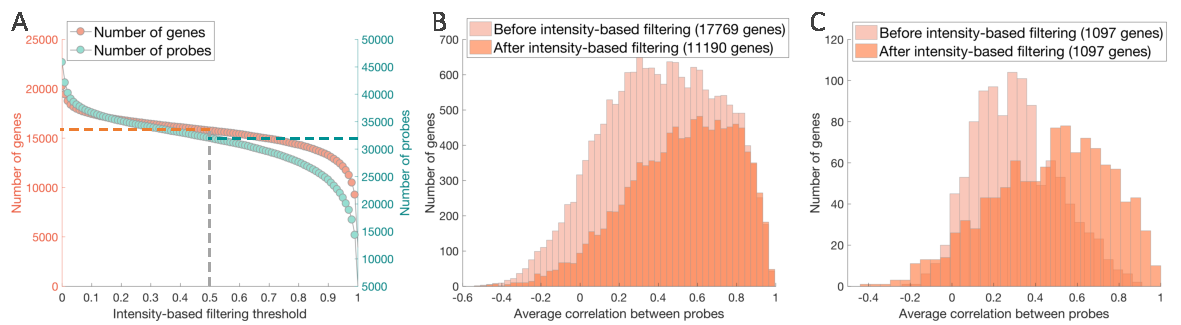
\includegraphics[width=1\textwidth]{Chapter4/Ch4Fig3.pdf}
\caption{\textbf{Intensity-based filtering (IBF) is consistent with an increase in a real expression signal, increasing the average inter-probe correlation for individual genes.} A) The number of probes and genes as a function of filtering threshold: $x$ axis – the minimum proportion of samples with expression values exceeding the background; $y$ axis – the number of probes and genes retained. Dotted lines correspond to the number of probes and genes retained after $50\%$ filtering threshold was applied.
B) Average correlation between expression values measured using all available probes for the same gene: light orange --- original set of \num{17769} genes with more than $1$ probe; dark orange – \num{11190} gene set after intensity-based filtering with more than one probe, where probes for which $50\%$ of samples do not survive IBF are removed.
C) Distributions of average correlations between expression values measured using all available probes for the same gene that demonstrated any change after IBF (\num{1097} genes, or $\sim10\%$ genes with multiple probes). }

\label{fig:Ch4Fig3}
\end{figure}

\subsection{Step 3. Probe selection}

Multiple probes can be used to measure the expression level of a single gene at different exons (segments of RNA molecules that code for a protein or peptide sequence), which can increase the reliability of the measurement. After performing re-annotation and IBF, $71\%$ genes in the AHBA were measured with at least two probes (compared to $93\%$ in the original data). One might expect that probes measuring the expression of the same gene should show consistent expression patterns, but this is not always the case. Differences between probes measuring the same gene can arise from different sources, including errors in probe sequences immobilised on the array during manufacturing; errors in mapping probe sequences to mRNA transcripts; inaccuracies in probe-to-gene annotations; probe-specific differences in hybridization specificity; and multiple splice variants of specific genes [for further details, see \citet{Liu2010}, and \citep{Jaksik2015}]. We find that, even after IBF, the correlation between probes measuring the expression levels of the same gene is $\rho < 0.3$ for more than $20\%$ of genes (Figure \ref{fig:Ch4Fig3}B). Investigators have used different strategies to derive a representative measure of gene expression some of which are summarized in Table \ref{Table2}.

\begin{table}[h!]
\caption{Methods used for deriving an estimate of gene expression in cases where multiple probes are available for the same gene.}
\label{Table2}
\resizebox{\textwidth}{!}{%
\begin{tabular}{ll}
\hline
\multicolumn{1}{c}{\textbf{Method}} & \multicolumn{1}{c}{\textbf{Description}} \\ \hline
Mean & \begin{tabular}[c]{@{}l@{}}
Calculate the mean of all available probes for a gene. \\ \citet{Tan2013,French2015,Eising2016,Krienen2016} \\ \citet{Vertes2016b,Whitaker2016a,Negi2017,McColgan2018} \end{tabular} \\ \hline
Max intensity & \begin{tabular}[c]{@{}l@{}}
Select probe with the highest expression level. \citet{Romero-Garcia2018} \end{tabular} \\ \hline
Variance & \begin{tabular}[c]{@{}l@{}}
Select the probe with the highest variance across brain regions. \citet{Negi2017} \end{tabular} \\ \hline
PC & \begin{tabular}[c]{@{}l@{}}
Select the probe with the highest loading onto the first principal component of probes. \citet{Parkes2017} \end{tabular} \\ \hline
Differential stability (DS) & \begin{tabular}[c]{@{}l@{}}
Select the probe with most consistent pattern of regional variations cross the six donor \\ brains, as quantified using a measure called Differential Stability (DS). \\ \citet{Hawrylycz2015,Kirsch2016a} \end{tabular} \\ \hline
Correlation variance/intensity & \begin{tabular}[c]{@{}l@{}}
Select the probe with the highest average correlation to other probes$^{a}$ for \textgreater{}2 probes; \\ select the probe with maximum variance (correlation variance) or maximum intensity \\ (correlation intensity) when only 2 probes available. \citet{Hawrylycz2012,Hawrylycz2015,Myers2015a}\\ \citet{Burt2018,Forest2017,Anderson2018} \end{tabular} \\ \hline
Sequence mismatches & \begin{tabular}[c]{@{}l@{}}
Select the probe with fewest sequence mismatches, or the probe with highest standard deviation \\ if \textgreater 1 probe have the same number of mismatches$^{b}$. \citet{Richiardi2015} \end{tabular} \\ \hline
\end{tabular}}
\begin{tablenotes}
     \item[1] $^{a}$ This measure is implemented in the R function ‘collapseRows’ from WGCNA package \citep{Miller2011}. Here we used a custom implementation of this function that was applied for samples within each brain separately in order to account for potential inter-individual differences in gene expression (discussed in step $5$).
     \item[2] $^{b}$ Sequence mismatch is defined by Re-annotator software as the difference between probe sequence and the reference genome sequencing data. Considering that $\sim93\%$ probes were re-annotated without any mismatches, the overwhelming majority of probes will be chosen applying the highest standard deviation criteria and resemble maximum variance selection approach. Therefore, this probe selection criteria was not implemented separately and is not presented in the probe selection comparison plots.
   \end{tablenotes}
\end{table}

To evaluate how the gene expression measures vary under different probe selection methods, we estimated, a single summary measure of expression for each gene indexed by multiple probes, according to one of the methods listed in Table \ref{Table2}. We also evaluated a few other methods beyond those used in the published literature, such as selecting the probe with maximum coefficient of variation across samples (CV), or the probe with the highest proportion of samples with expression levels exceeding background noise (signal proportion). In addition, we included random probe selection (averaged over $100$ repeats) for comparison. We then took the expression vector of each gene across tissue samples and computed the Spearman rank correlation coefficients  between these vectors estimated for each possible pair of methods.

Figure \ref{fig:Ch4Fig4}A shows the average correlation between expression measures selected using different criteria, averaged across \num{17769} genes assayed by multiple probes. Since most studies using the AHBA do not report using IBF, we show results for unfiltered data (similar results were obtained using IBF, see Figure \ref{fig:Ch4Sfig1}). The average correlation coefficients between probe selection methods range between $0.5 < \bar{\rho} < 0.98$, indicating that the probe selection method can have a major impact on expression estimates. The method of summarizing the expression measures for a gene as the mean across all available probes is the most highly correlated, on average, to all the other methods. Variance-related methods [coefficient of variation, maximum variance, correlation-variance and highest loading on first PC of non-normalized data \citep{Parkes2017}] are similar to each other, but different to other methods. Consistency (DS) and intensity (max intensity, signal proportion and correlation-intensity) related methods, on the other hand, are more correlated with each other. Notably, the correlations between gene expression measures selected based on the highest CV compared to the consistency/intensity-related criteria are much lower than resulting from the random probe selection strategy, indicating that these methods favour dissimilar properties of expression measures for probe selection. A more detailed discussion of these results is presented in \ref{app:AppendixCh4_3}.

\begin{figure}[h!]
  \centering
    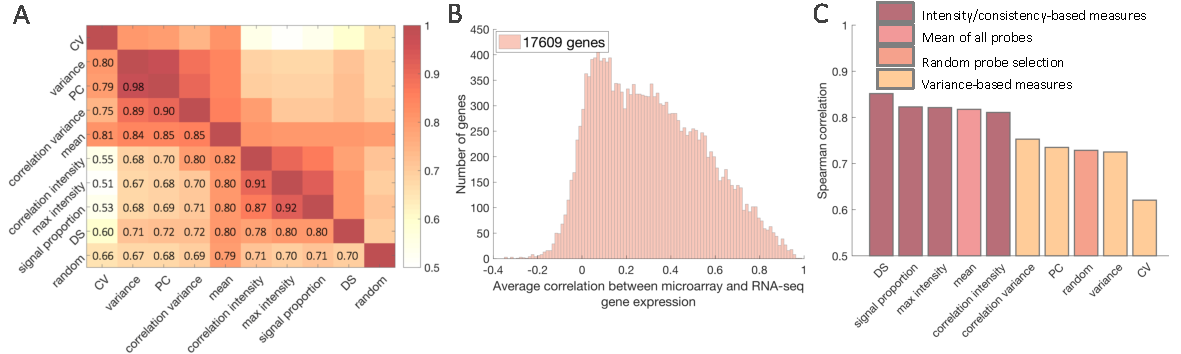
\includegraphics[width=1\textwidth]{Chapter4/Ch4Fig4.pdf}
\caption{\textbf{The probe selection method can have a large effect on resulting gene expression estimates.}
A) Mean Spearman correlation coefficient of expression levels across \num{17769} genes with multiple probe annotations, using a range of different probe selection methods: CV, variance, PC, signal proportion, DS, correlation variance, correlation intensity, mean (see Table \ref{Table2}) or selecting a representative probe at random (correlation values averaged over $100$ runs).
B) The distribution of Spearman correlation values between microarray and RNA-seq expression data for genes that are present in both datasets. When multiple probes for a gene are available, the maximum correlation value between probes was selected.
C) Average correlation between probes selected using RNA-seq (by selecting the probe that is most correlated with the RNA-seq data) and other methods (ordered by decreasing values), based on \num{10221} genes that: (i) had more than one probe available; (ii) were present in both microarray and RNA-seq datasets; (iii) were correlated to RNA-seq ($\rho > 0.2$, Spearman’s rank correlation) to ensure that RNA-seq based probe selection provides a meaningful estimate in regards to the microarray data.}
\label{fig:Ch4Fig4}
\end{figure}

The lack of a gold standard makes it difficult to choose between different probe selection options. One strategy is to use RNA-seq data as an external reference \citep{Miller2014a}. Comparing expression values for matching structures in each of the two brains allows us to select probes that correlate most strongly with RNA-seq, providing an additional quality control measure to cross-validate probe selection.

Considering that \num{17609} of the \num{20232} genes in the microarray data have RNA-seq measures, we first aimed to evaluate whether excluding the $\sim13\%$ of genes that do not overlap between the datasets would eliminate brain-relevant genes. We verified this using over-representation analysis ORA, which is designed to identify statistically over-represented gene categories \citep{Gillis2010}: the genes removed are not enriched in brain-specific functions but rather are related to generic processes such as septin assembly and organization, as well as the negative regulation of RNA splicing (see supplementary file enrichmentExpression.csv for results and \ref{app:AppendixCh4_2} for more details).

We then examined the correlations between microarray and RNA-seq expression measures in the \num{17609} genes that overlap between both RNA-seq and microarray datasets across $112$ brain regions, as shown in Figure \ref{fig:Ch4Fig4}B. Most correlations are low, with $52\%$ of genes exhibiting a correlation $\rho < 0.3$ and only $23\%$ genes exhibiting a correlation $\rho > 0.5$. This divergence between RNA-seq and microarray is likely to be caused by inaccuracies in the microarray measurements. Using GSR analysis \citep{Gillis2010}, we find that genes with higher correlations between microarray and RNA-seq are related to neuronal connectivity and communication related processes with categories such as ‘transmission of nerve impulse’, ’ensheathment of neurons’, ‘myelination’ and ‘glial cell development’ demonstrating the strongest enrichment (see supplementary file enrichmentExpression.csv for results and \ref{app:AppendixCh4_2} text for more details). This analysis suggests that RNA-seq data can be used as a reference to select brain-relevant and reliably measured genes.

Figure \ref{fig:Ch4Fig4}C shows that, compared to other probe selection methods, RNA-seq demonstrates the highest similarity to intensity/consistency-based approaches ($\rho > 0.8$, Spearman’s rank correlation), with DS showing the highest correlation. In contrast, variance-based methods are no more similar to the RNA-seq measures than random probe selection ($\rho < 0.75$, Spearman’s rank correlation). Given that RNA-seq data is only available for a limited number of samples (with only $87\%$ of genes being represented), and the data come from only two of the six donor brains in the AHBA, Figure \ref{fig:Ch4Fig4}C indicates that DS may be a reasonable alternative method for probe selection that can be generalized to the full AHBA.

\subsection{Step 4. Assigning samples to brain regions}

The AHBA provides gene expression data for multiple spatially localized tissue samples (Figure \ref{fig:Ch4Fig1}). When relating such data to macroscopic IDPs, it is necessary to generate some mapping between the spatial location of each tissue sample and the particular spatial unit of analysis (e.g., voxel, brain region) used to construct the IDP. This mapping is facilitated by the AHBA including an MNI coordinate (and voxel coordinate) for each tissue sample, and MRI data acquired for each individual brain contained in the AHBA. Each tissue sample is also associated with an anatomical structure ID, which can be related to corresponding higher order structures using the Allen Institute anatomical ontology, allowing brain structures to be identified at different resolution scales.

Existing studies have used several approaches to map tissue samples to regions-of-interest (ROIs) in imaging data.
One strategy has been to match samples to structures based on the name of a given anatomical sample. The simplest approach is to use the anatomical structure names provided by the AHBA [see \citet{AHBAdoc,Tan2013,Myers2015a,Chen2016,Kirsch2016a,Hecker2017,Lee2017a,Negi2017}], but these regions do not directly correspond to brain parcellations typically used in imaging analyses, so precise alignment with imaging data can be difficult. An alternative approach is to use the MNI (or voxel) coordinates of each sample \citep{Goyal2014,Cioli2014b,French2015,Richiardi2015,Komorowski2016,Krienen2016,Rizzo2016,Burt2018,Parkes2017,Romme2017,Shin2017,Anderson2018,Romero-Garcia2018}.
It is possible to either assign samples to brain regions in a single parcellation defined in MNI space \citep{Krienen2016,Keo2017,Parkes2017,Romme2017}, or to assign samples to regions based on parcellations of each individual AHBA brain \citep{Romero-Garcia2018}. The former approach is simpler, but a characteristic of the AHBA is that the MNI coordinates provided for each tissue sample are based on spatial normalizations that were tailored to each individual brain. Specifically, two of the AHBA brains were scanned \textit{in cranio} and normalized to MNI space via a linear transformation, whereas the other four were acquired \textit{ex cranio} and normalized using an affine followed by a non-linear transformation [for details see \citep{AHBAdoc}] with the deformation fields also being smoothed to facilitate matching the images to Nissl stains. These differences across brains will influence the accuracy of the normalization across the six brains, which is compounded by differences in tissue distortion that occurred during sample handling and processing.

To overcome these issues, a parcellation scheme can be applied to each individual donor brain. This method can more accurately account for individual differences in anatomy but is contingent on being able to generate appropriate transformations between native and MNI space for an accurate parcellation. For cortex, the accuracy of the parcellation can be greatly enhanced by parcellating and normalizing the surface while the parcellation of non-cortical areas requires volumetric normalization. In our own work, we have been able to segment the cortical surfaces of the six AHBA brains with reasonable accuracy (assessed by visual inspection), and we supply four different volumetric parcellations mapped at different resolutions to each brain using FreeSurfer: the Desikan-Killany \citep{Desikan2006}, comprising $34$ nodes per hemisphere, the group-level HCPMMP1 \citep{Glasser2016} comprising $180$ nodes per hemisphere, and two random parcellations comprising $100$ and $250$ nodes per hemisphere, respectively.

Once a particular parcellation has been generated, tissue samples should be assigned to the nearest region of the parcellation. In this assignment, a threshold can also be applied, to avoid assigning samples beyond a certain distance. The distance between sample and region is commonly estimated as the Euclidean distance in 3D space. This sample-region distance has been computed in different ways, including representing a region in space by its centroid coordinate \citep{Vertes2016b,Whitaker2016a,McColgan2018}, or taking the minimum distance between the sample and any voxel in the region \citep{French2015,Parkes2017,Romme2017}. The latter approach is more accurate, given that regions in any given parcellation vary in size and folded geometry (e.g., Figure \ref{fig:Ch4Fig5}A).

\begin{figure}[h!]
  \centering
    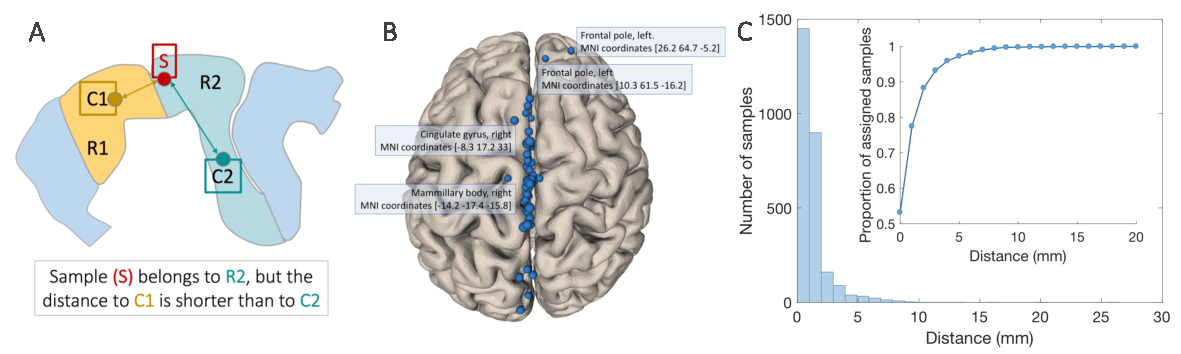
\includegraphics[width=1\textwidth]{Chapter4/Ch4Fig5.pdf}
\caption{\textbf{Methods for assigning localized tissue samples to matching regions in a brain parcellation are sensitive to the metric used to define sample–region distances, the distance threshold used, and the use of anatomical annotations on individual samples.}
A) Schematic representation of sample assignment when a sample is assigned to the closest ROI centroid. A given sample belongs to region R2 but is closer to the centroid (C1) of region R1 than the centroid (C2) of R2, resulting in an erroneous assignment.
B) Schematic representation of samples that were assigned to a hemisphere that differed from the annotations provided with their MNI coordinates.
C) Sample assignment using distance thresholds: the number of samples across all six brains within a given distance from a parcellation region. Insert shows the proportion of assigned samples as a function of distance threshold. At a \num{2} mm distance threshold, $\sim$\num{90}\%  of tissue samples can be matched to a region in the parcellation. }
\label{fig:Ch4Fig5}
\end{figure}

In this process of assigning samples to regions, errors can occur if the mapping is not done separately for (i) broad anatomical division (cortex, subcortex, cerebellum and so on); and (ii) left and right hemispheres. That is, cortical samples listed as coming from the left hemisphere in the AHBA ontology should only be mapped to left cortical voxels (as samples were taken from annatomically known positions in the brain), right subcortical or cerebellar samples to right subcortical/cerebellar voxels and so on.

In our own experience, we have observed that subcortical samples (as indicated by AHBA ontology) can be mapped to cortical regions of the parcellation as a cortical voxel may be closer (or visa versa). Similarly, if no separation between hemispheres is performed, $58$ out of \num{2748} cortical and subcortical samples are assigned to an incorrect side of the brain when using the Desikan-Killany \citep{Desikan2006} parcellation (Figure \ref{fig:Ch4Fig5}B). While the majority of those samples are very close to the midline, several are clearly incorrectly mapped to the stereotaxic space, such as two samples in the frontal pole, which are assigned to the left side of the brain according to the AHBA annotations but have a positive MNI $x$-coordinate. The same is true for some samples from the mammillary body and cingulate gyrus, which are labelled as coming from the right hemisphere but have negative MNI $x$-coordinates (Figure \ref{fig:Ch4Fig5}B). To avoid potential mistakes, samples with mismatching assignments should be excluded. In addition, the AHBA ontology classifies hippocampus as a part of the cerebral cortex while most neuroimaging tools do not. Given the differences in gene expression between the neocortex and allocortex, including hippocampal samples when integrating information from the cortical sheet may give misleading results.

A second consideration is to set a distance threshold for assigning samples to regions, to ensure that samples further than a given threshold away from the parcellation will not be assigned \citep{Romero-Garcia2018}. As shown in Figure \ref{fig:Ch4Fig5}C, only around $50\%$ of samples are directly mapped to a parcellation when using the Desikan-Killany \citep{Desikan2006} parcellation (i.e., their coordinates correspond to a voxel inside the parcellation). Increasing the distance threshold will allow some tolerance for small errors in spatial normalization. For example, \citet{Romero-Garcia2018} implemented distance-constrained sample assignment by extending the parcellation into the white matter in order to include those cortical samples that have not been directly mapped to the parcellation. Figure \ref{fig:Ch4Fig5}C shows that assigning samples that are up to $2$ mm away from any voxel in the parcellation increases the proportion of assigned samples to almost $90\%$, with additional increases in the distance threshold yielding only minor gains in the number of assigned samples. Therefore, we use a $2$ mm distance threshold in our analyses.

An important consideration regarding sample assignment arises from the fact that only two out of six brains were sampled from both hemispheres and four brains have samples collected only in the left. This sparse sampling should be carefully considered when combining data across donors. Restricting analyses to the left hemisphere will minimize variability across regions (and hemispheres) in terms of the number of samples available. However, if a whole-brain analysis is desired, such variability should be carefully studied to ensure that it does not impact one’s findings. In the \ref{app:AppendixCh4_4}, we provide information on the number of samples assigned to four different parcellations. One way to deal with limited anatomical coverage in the AHBA is to infer missing expression values based on some model of the data. For example, \citet{Gryglewski2018} built a Gaussian process regression model using a weighted linear combination of the nearest samples to infer the missing expression value at a particular location. Validation of model predictions in new data would support its use in extending the coverage of the current AHBA.

\subsection*{Step 5. Six brains, one atlas: accounting for individual variability}

The AHBA is often used to represent a general transcriptomic profile of the adult human brain. However, it is comprised of data taken from people aged $24$ to $57$ years, of different ethnicities, sexes, medical histories, causes of death, and post-mortem intervals (Table \ref{Table3}). Many of these factors can impact gene expression \citep{Fraser2005,Berchtold2008,Kumar2013,Trabzuni2013}. One way to address this brain-specific variance is to conduct analyses separately in each brain. However, spatial coverage of different brain areas in the AHBA varies from person to person. Therefore, collapsing samples from all brains to derive a single atlas with maximum spatial coverage. In this case, an appropriate correction for donor-specific transcriptomic patterns is required.


\begin{table}[h!]
\caption{Information about the six adult donors in AHBA.}
\label{Table3}
\resizebox{\textwidth}{!}{%
\begin{tabular}{llllll}
\hline
\multicolumn{1}{c}{\textbf{Donor}} & \multicolumn{1}{c}{\textbf{Age}} & \multicolumn{1}{c}{\textbf{Sex}} & \multicolumn{1}{c}{\textbf{Ethnicity}} & \multicolumn{1}{c}{\textbf{Medical conditions}} & \multicolumn{1}{c}{\textbf{Post-mortem interval$^{a}$}} \\ \hline
H0351\_2001$^{b}$ & 24  & Male   & \makecell{African \\ American} & \begin{tabular}[c]{@{}l@{}}History of asthma \end{tabular} & 23 hours \\ \hline
H0351\_2002$^{b}$ & 39  & Male   & \makecell{African \\American} & \begin{tabular}[c]{@{}l@{}}Possible small pituitary adenoma; \\single neurofibrillary tangle in entorhinal cortex \end{tabular}                                                                                                      & 10 hours \\ \hline
H0351\_1009 & 57  & Male   & Caucasian        & \begin{tabular}[c]{@{}l@{}}History of atherosclerotic cardiovascular disease \end{tabular}                                                                                                                                        & 25.5 hours            \\
\hline
H0351\_1012 & 31  & Male   & Caucasian        & \begin{tabular}[c]{@{}l@{}}Sudden cardiac arrest; benign spindle cell \\ proliferation and dystrophic calcification \\ in temporal horn of lateral ventricle \end{tabular}                                                               & 17.5 hours            \\
\hline
H0351\_1015 & 49  & Female & Hispanic         & \begin{tabular}[c]{@{}l@{}}Splenectomy, hypothyroidism treated with Levothroid;\\ modest numbers of hemosiderin laden macrophages \\ noted in Virchow-Robin spaces in parietal and occipital \\ lobes, mild arteriosclerosis \end{tabular}
& 30 hours              \\
\hline
H0351\_1016 & 55  & Male   & Caucasian        & \begin{tabular}[c]{@{}l@{}}Coronary artery atherosclerosis, prescriptions \\ for clotting and high cholesterol                                                                                                         \end{tabular} & 18 hours              \\
\hline
\end{tabular}}
\begin{tablenotes}
     \item[1] $^{a}$ Post-mortem interval is defined as the time period from the time of death to the time the tissue is frozen.
     \item[1] $^{b}$ These donors have tissue samples collected across both left and right hemispheres while all the other donors have samples only from within the left hemisphere.
   \end{tablenotes}
\end{table}

The Allen Institute applied a range of data normalization procedures to remove batch effects and artefactual inter-individual differences. Nonetheless, residual inter-individual differences remain (Figure \ref{fig:Ch4Fig6}A). While a number of studies account for the additional inter-individual differences between donor brains through subject-specific normalization prior to aggregation \citep{Richiardi2015,Whitaker2016a,Vertes2016b,Negi2017,Liu2017,Romero-Garcia2018,Burt2018,McColgan2018}, some perform normalization after aggregating across subjects \citep{Parkes2017} or do not explicitly specify inter-subject normalisation \citep{Veronese2016}. Here we investigated whether intrinsic inter-individual differences in gene expression are able to discriminate individual donor brains by projecting all tissue samples from all six brains into a two-dimensional transcriptional principal components space. Figure \ref{fig:Ch4Fig6}A plots loadings of each cortical tissue sample on the first two principal components of gene expression for all six donors (for the whole brain see Figure \ref{fig:Ch4Sfig5}). This unsupervised projection of samples into gene expression space captures the latent dimensions of variance between all samples and broadly separates the six donors (regardless of where a tissue is located in the brain), indicating that each donor has a distinctive gene expression profile. In other words, while the data normalization procedures applied by the Allen Institute prior to data release removed batch effects and artefactual inter-individual differences, a considerable degree of intrinsic donor-specific variance remains and must be accounted for in order to perform valid data aggregation.

\begin{figure}[h!]
  \centering
    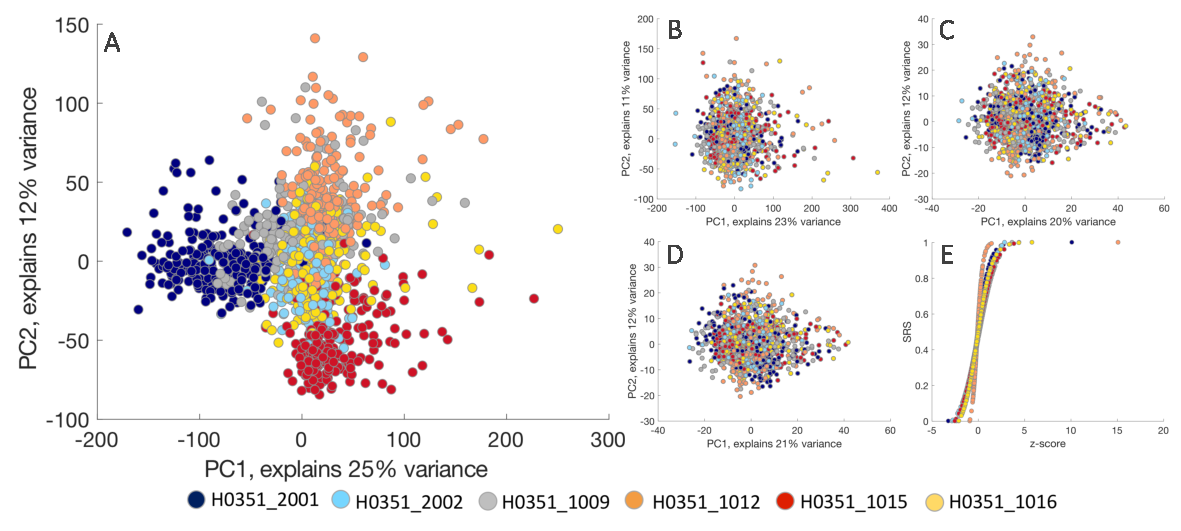
\includegraphics[width=1\textwidth]{Chapter4/Ch4Fig6.pdf}
\caption{\textbf{Appropriate normalization can remove donor-specific variability in gene expression.}
A) Non-normalized gene expression data in principal component (PC) space. Data from different donors are represented in different colours. Samples from different subjects occupy different parts of the low-dimensional gene expression space. Panels B,C represent gene expression data in principal component space normalized separately for each subject using $z$-scores
(B) or the scaled robust sigmoid (SRS) transform (C). Panel D shows gene expression data in principal component space after applying \textit{limma} batch effect removal \citep{Ritchie2015} on cross-subject aggregated data, followed by SRS normalization. After normalization (B,C,D), samples no longer segregate by donor. E) Correlations between normalized expression values ($z$-score \textit{vs} SRS) for the ZZZ3 gene (chosen for visualization purposes).
Each dot represents a normalized expression value for ZZZ3 gene across samples, and different colours correspond to different subjects. The $z$-score normalization results in extreme values being assigned to outliers, therefore producing different scales for subjects and complicating direct comparison of values.
This example demonstrates how outliers in the data can affect the scaling for different subjects: using $z$-score normalization results in different scales for different subjects with normalized values ranging from approximately $–5$ to $5$ for four out of six subjects, whereas subjects H0351\_1012 (orange) and H0351\_2001 (dark blue) have a much wider range. In comparison, SRS produces normalized expression values on the same scale for each subject without being affected by outliers.
Representations in principal component space are based on \num{10028} genes, with representative probes chosen based on correlation to RNA-seq data. }
\label{fig:Ch4Fig6}
\end{figure}

One approach for addressing donor-specific effects is to perform a leave-one-out analysis, where the analysis is repeated six times, excluding one of the brains at each iteration  \citep{Parkes2017,McColgan2018}. Such an approach can rule out the undue influence of any single brain, provided that the results are consistent across iterations. A more direct way of eliminating the inter-individual differences in expression measures is to normalize the gene expression data separately for each subject \citep{Richiardi2015,Whitaker2016a,Vertes2016b,Rizzo2016,Liu2017,Negi2017,Burt2018,McColgan2018,Romero-Garcia2018a}. With this approach, each gene’s expression values are normalized across regions separately for each donor in order to reflect the relative expression of each gene across regions, within a given brain (Figure \ref{fig:Ch4Fig6}B-D). A desirable normalization procedure should offer robustness to outlying values and quantify expression on the same scale across donors to enable direct comparison. Most studies using AHBA have used $z$-score normalization \citep{Rizzo2016,Whitaker2016a,Vertes2016b,Negi2017,Romero-Garcia2018a},

\begin{equation}
    \label{eqn:eq1}
    x_\mathrm{norm} = \frac{x_\mathrm{\textit{i}}-\overline{x}}{\sigma},
\end{equation}
where $\overline{x}$ represents the mean, $\sigma$ represents the standard deviation and $x_\mathrm{\textit{i}}$ --- the expression value of a gene in a single sample. The estimates of $\overline{x}$ and $\sigma$ are appropriate for symmetric distributions, whereas gene expression distributions across brain samples are often non-symmetric, and can contain outliers, which can bias these summary statistics. Figure \ref{fig:Ch4Fig6}E demonstrates the sensitivity of $z$-score normalization to the outlying values.
A variety of outlier-robust normalizations exist such as Hampel hyperbolic tangent transformation, however here we focus on a variant of a normalization method used by \citet{Fulcher2016}, the scaled robust sigmoid (SRS) normalization \citep{Fulcher2013}. This approach normalizes gene expression values based on an outlier-robust sigmoid function,

\begin{equation}
    \label{eqn:eq2}
    x_\mathrm{y} = \frac{1}{1+\mathrm{exp}({\frac{-(x_\mathrm{\textit{i}}-\left\langle x \right\rangle)}{\mathrm{IQR}/1.35}})},
\end{equation}
where $\left\langle x \right\rangle$ represents the median and $\mathrm{IQR}$ represents the interquantile range, before rescaling normalized values to a unit interval,

\begin{equation}
    \label{eqn:eq3}
    x_\mathrm{norm} = \frac{x_\mathrm{y}-\mathrm{min(x)}}{\mathrm{max(x)}-\mathrm{min(x)}}.
\end{equation}

This normalization is robust to outliers and ensures equivalent scaling of expression values for each person. Figures \ref{fig:Ch4Fig6}C and E show the effectiveness of SRS in dealing with outliers and scaling. Other strategies for removing donor-specific effects involve using linear models applied to cross-donor combined data. For example, donor-specific effects can be treated as an additional batch effect and removed via linear modelling using the R/Bioconductor software package \textit{limma} \citep{Ritchie2015}. While this approach removes inter-individual differences in gene expression, the linear model is sensitive to outliers. This correction in turn can be followed by SRS normalization to minimize the influence of outliers (Figure \ref{fig:Ch4Fig6}D).

To account for potential between-sample differences in gene expression, \citet{Burt2018} introduced within-sample normalization across genes before subject-specific normalization across samples (see Figure \ref{fig:Ch4Sfig6}). Indeed, some samples can show a markedly different expression profile (extremely low or high values across all genes) from other samples in close spatial proximity, potentially due to measurement artefacts. The influence of these artefacts can be minimized by applying within-sample cross-gene normalization to quantify relative expression levels within a given sample, before normalizing across samples. To quantify the effect of the initial within-sample normalization, we calculated the correlations between expression values across genes and samples in two cases: i) when only cross-sample normalization for each gene was applied; ii) when both cross-gene normalization within sample as well as cross-sample normalization for each gene were applied. While the correlation values were relatively high ($\mathrm{median_\mathrm{sample}}(r) =  0.97$, $\mathrm{IQR} = 0.04$; $\mathrm{median_\mathrm{gene}}(r) = 0.86$, $\mathrm{IQR} = 0.1$), based on visual inspection, the initial within sample normalization was beneficial in reducing potential measurement artefacts in the data.

One additional consideration is that the spatial distribution of tissue samples across individual brains in the AHBA is not uniform. As such, different brains can contribute a different number of samples to any given brain region (Figure \ref{fig:Ch4Fig1} and Figure \ref{fig:Ch4Sfig7}). In light of this variability, we have two choices: we can either average all samples falling within a region, meaning that the average may be driven by a subset of individuals who have more samples localized to that region, or we can average at the level of each individual donor brain before aggregating across people (Figure \ref{fig:Ch4Sfig7}). The latter approach ensures that each donor makes an equal contribution to the mean, provided that all genes are normalized to the same scale. While the choice of inter-subject averaging does not significantly impact whole-brain analyses, it might have a more pronounced effect if the analysis is focused on a particular region where samples are not evenly distributed across donors (for a more detailed explanation see Figure \ref{fig:Ch4Sfig7}).

\subsection{Step 6. Gene filtering}

The AHBA consists of more than \num{20000} unique genes, of which only a fraction is expected to show consistent regional variations in expression across the brain. Many analyses interested in transcriptomic signatures of IDPs will be primarily interested in these brain-specific genes. Various methods for pre-selecting genes of interest have been adopted, including selecting: (i) disease-specific genes \citep{Rittman2016,Romme2017,Yokoyama2017a}, (ii) genes related to a priori hypotheses \citep{Goyal2014,Komorowski2016,Krienen2016,Acevedo-Triana2017}, (iii) genes that are expressed consistently across all six AHBA brains, as quantified using the DS measure \citep{Hawrylycz2015}, or (iv) demonstrate consistent expression between different gene expression datasets \citep{Shin2017}. Genes with high DS values demonstrate consistent patterns of regional variation in expression across the six AHBA subjects, and have been shown to be enriched for brain-related biological functions \citep{Hawrylycz2015}. Filtering based on DS thus offers a more targeted approach for investigating relationships between IDPs and gene expression compared to whole-genome analysis.

The selection of disease-specific genes is traditionally based on previous GWAS studies \citep{Satake2009,Simon-Sanchez2009,Hoglinger2011,Ferrari2014,Ripke2014a,Kouri2015}, while gene selection based on an \textit{a priori} hypothesis can depend on other factors such as a specific involvement in clinical disorders \citep{Komorowski2016,Acevedo-Triana2017}. One particular set of 19 genes demonstrating a selective enrichment in the upper layers of the human cortex compared to mouse [Human Supragranular Enriched (HSE) genes] has been extensively investigated and was found to be related to measures of functional connectivity \citep{Krienen2016} and brain network topology \citep{Vertes2016b,Romero-Garcia2018}.

\subsection{Step 7. Accounting for spatial effects}

The application of steps 1 to 6 results in a processed region $\times$ gene matrix of transcription level values, which can be used for further analyses. Typically, the data are linked to IDPs at either the regional level, or at the level of pairs of regions [i.e., patterns of correlated gene expression (CGE) between pairs of brain regions are related to pair-wise measures of structural or functional connectivity between those regions \citep{Fornito2019}]. In both cases, we seek to understand how spatial variations in gene expression or CGE relate to spatial variations in the IDP. One complicating factor is that cortical regions that are located in close proximity are more likely to share similar gene expression patterns \citep{Richiardi2015,Krienen2016,Vertes2016b,Pantazatos2017,Richiardi2017}. A similar spatial autocorrelation of gene expression has been reported in the mouse brain \citep{Fulcher2016} and in the head of the nematode \textit{C. elegans} \citep{Arnatkeviciute2018}.

In some respects, this distance-dependence of gene expression is an interesting and physiologically meaningful trend that warrants further investigation [for a review, see \citep{Fornito2019}]. However, if an IDP varies across the brain in a manner that reproduces a spatial gradient in gene expression, any apparent association between the IDP and gene expression measures may be driven by low-order spatial effects. Depending on the research question, especially when a direct relationship between an IDP and gene expression is evaluated, it is important to confirm that the identified association is stronger than what would be expected based on the spatial autocorrelation properties of gene expression (if such an effect is claimed). For example, a researcher may wish to show that CGE is higher between nodes belonging to the same brain functional network. As spatially adjacent regions are more likely belong to the same functional system, such an effect may simply be driven by their separation distance rather than their functional identity. If one wishes to conclude that elevated CGE is related specifically to functional network affiliation, then the influence of spatial separation on CGE must be addressed. Indeed, this has been a topic of some debate in the literature \citep{Richiardi2015,Pantazatos2017,Richiardi2017}.

A critical first step in understanding spatial biases in gene expression is to define distances between brain regions. These distances can be estimated by (i) calculating the Euclidean distance between regions; (ii) estimating the shortest distance within the grey matter volume; or (iii) estimating the shortest distance on the cortical surface (Figure \ref{fig:Ch4Fig7}), see \ref{app:AppendixCh4_5} for more details. The Euclidean distance is the simplest method, but it approximates distances as straight lines that do not respect cortical geometry. Calculating distances within the grey matter volume or on the cortical surface present a more biologically valid approach, as distances are constrained by cortical geometry. A comparison of these methods, shown in Figure \ref{fig:Ch4Fig7}D, demonstrates that evaluating the Euclidean distance results in shorter distances, on average, compared to other methods, while anatomically constrained volume and surface-based approaches yield similar distance estimates in cortex. Note that the Euclidean approach is easier to generalize for measuring distances to subcortex.

\begin{figure}[h!]
  \centering
    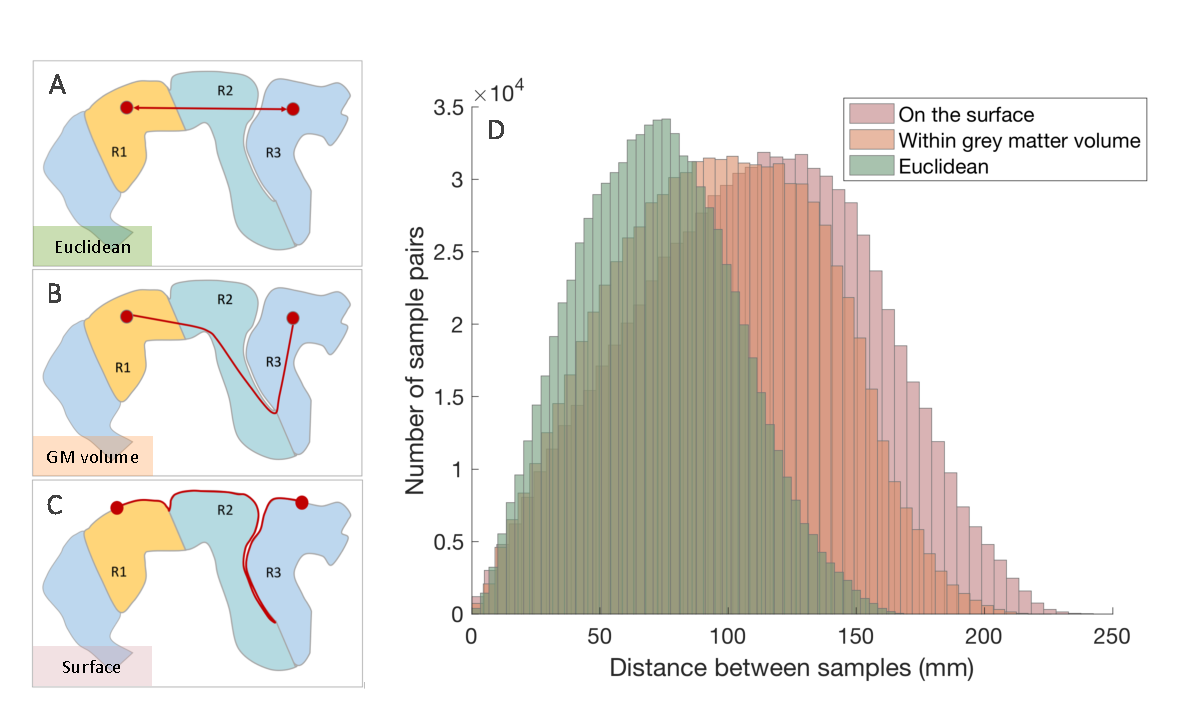
\includegraphics[width=1\textwidth]{Chapter4/Ch4Fig7.pdf}
\caption{\textbf{Distances between samples can be defined in different ways.}
Schematic representation of different approaches to calculate the distances between samples.
A) Euclidean distance, defined as the shortest distance between two points.
B) Distance within grey matter defined as the shortest distance within the grey matter volume. This measure is implemented by representing each voxel in the cortex as a node and creating a three-dimensional network where the shortest distances between brain regions are found using Dijkstra's algorithm \citep{Dijkstra1959}. The resulting distances will approximate the distances between regions within the cortical volume.
C) Distance on a mesh-based representation of the cortical surface, where gene expression samples are assigned to vertices in the mesh and the shortest distance is calculated as a shortest path between them. Both Euclidean and grey matter distances can be calculated using volumetric parcellation schemes, while estimating the distance on the cortical surface requires generating a surface-based cortical parcellation.
D) Distributions for pairwise sample distances calculated using the three approaches. Euclidean distance estimates are lower compared to both distances estimated within grey matter volume and on the surface. }
\label{fig:Ch4Fig7}
\end{figure}

Spatial effects are most easily examined in the context of analyses of correlated gene expression. Such analyses focus on patterns of pair-wise or multivariate transcriptional coupling between regions, where transcriptional coupling is estimated as a correlation between regional expression profiles. Such measures of CGE can then be related to some inter-regional IDP, such as a measure of functional or structural connectivity \citep{Richiardi2015,Fulcher2016,Arnatkeviciute2018}. Figure \ref{fig:Ch4Fig8}A shows that CGE decays sharply as a function of increasing spatial distance (on the pial surface) between regions in the cortex; relationships for other distance measures are qualitatively similar (see Figure \ref{fig:Ch4Sfig8}). In line with previous findings in different species \citep{Fulcher2016,Arnatkeviciute2018}, the dependence of CGE on distance can be approximated as an exponential (Figure \ref{fig:Ch4Fig8}A) and therefore the residuals of the exponential fit could be further used in the analyses (Figure \ref{fig:Ch4Fig8}B). Extending this relationship to the whole brain, including samples from both cortex and subcortex, is complicated by a strong anti-correlation between cortical and subcortical gene expression \citep{Hawrylycz2015}. Thus, separate normalization procedures for cortical and subcortical regions and corrections for different types of region pairs can be applied (see \ref{app:AppendixCh4_6} and Figure \ref{fig:Ch4Sfig9} for more details). Note also that the dependence of CGE on distance can vary as a function of the gene set and parcellation being used (see Figure \ref{fig:Ch4Sfig10}).

\begin{figure}[h]
  \centering
    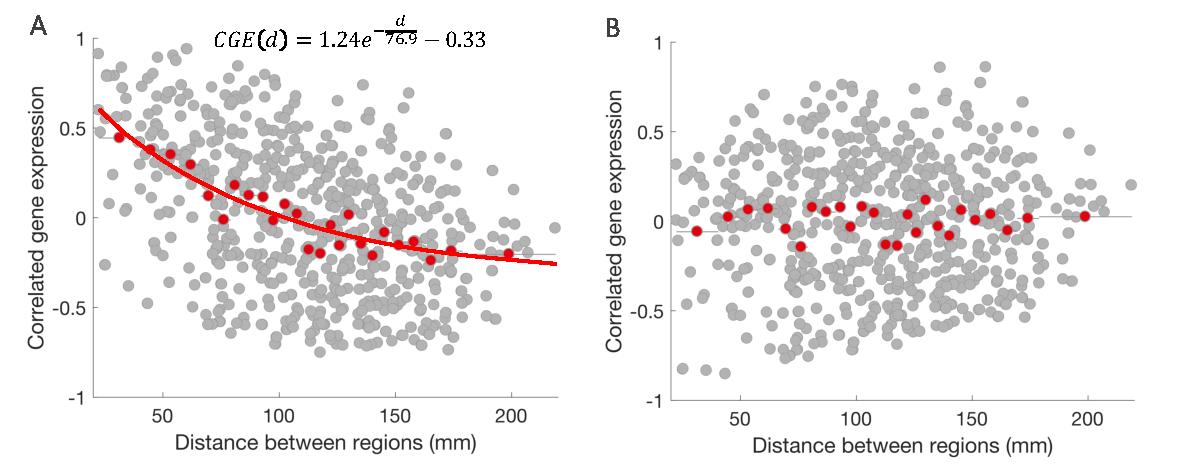
\includegraphics[width=1\textwidth]{Chapter4/Ch4Fig8.pdf}
\caption{\textbf{Characterizing the distance-dependence of gene expression data.}
A) CGE as a function of separation distance on the cortical surface. The red line represents an exponential fit $CGE(d) = 1.24e^{-d/76.9}-0.33$.
B) CGE residuals after removing the exponential trend. CGE between pairs of regions are represented in grey dots and red dots represent the mean value in $25$ equiprobable distance bins after the correction. CGE calculated using all \num{10027} genes (after intensity-based filtering and probe selection based on correlation to RNA-seq data).}
\label{fig:Ch4Fig8}
\end{figure}

Characterizing and removing distance dependence can be relatively straightforward in analyses of CGE. Addressing spatial relationships in analyses of regional gene expression can be more challenging since distance is defined between pairs of regions, whereas a regional expression value is a property of a single region. Some promising strategies to deal with this issue involve comparing observed findings relative to an appropriate null model. One class of methods uses spatially constrained permutation of the original data. Arbitrarily-defined regions are not independent from one another, so some spatial constraints are required to account for these dependencies during permutation. As an example, a block permutation algorithm implemented by \citet{Vertes2016b} accounted for spatial relationships between regions by aggregating areas into spatially contiguous subsets (blocks) according to the Desikan-Killiany atlas, and then permuting the resulting blocks rather than individual regions. \citet{Vasa2018} introduced a spatial permutation test based on the rotation of regional coordinates in the spherical projection, such that the relative spatial relationships between regions are preserved. Matching between original and rotated coordinates, therefore, allows the regional measure to be permuted while controlling for spatial contiguity and hemispheric symmetry. \citet{Burt2018} used a spatial lagged autocorrelation model to characterise the spatial dependency between observed gene expression values. Moreover, while these approaches provide some valid options, thorough evaluation of these null models is an important avenue of future work. While distance is perhaps the most obvious influence to consider correcting in expression analyses, other factors, such as regional variations in cytoarchitecture and cell density, are also relevant considerations \citep{Barbas2015,Burt2018}. The appropriateness of different corrections should be carefully motivated by the specific research question.

\begin{table}[H]
\caption{Recommendations and practical considerations for each data processing step.}
  \centering
    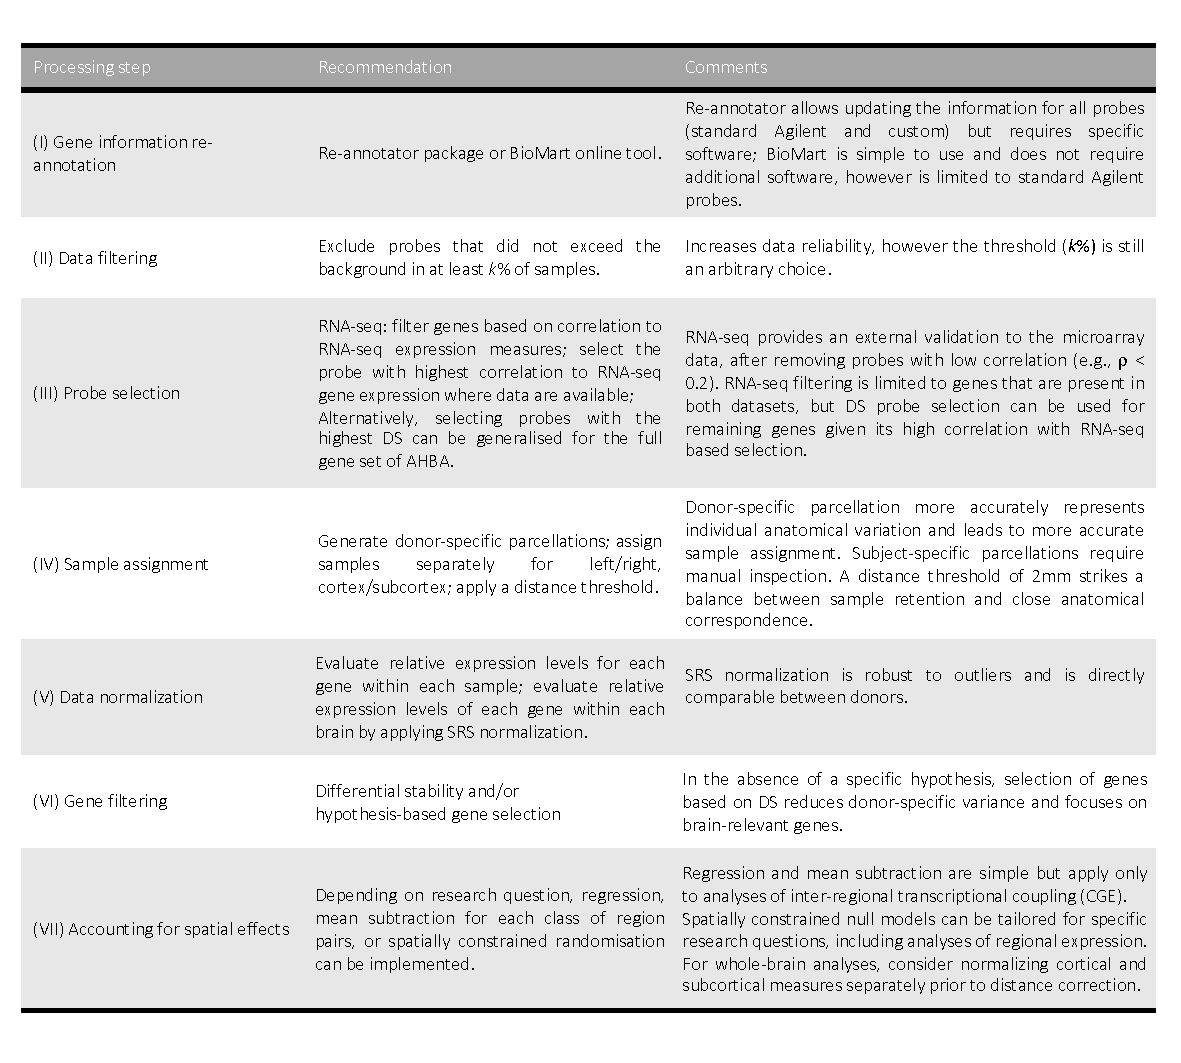
\includegraphics[width=1\textwidth]{Chapter4/Ch4Fig9.pdf}
\label{fig:Ch4Fig9}
\end{table}

\section{Conclusions}

Imaging transcriptomics provides an unprecedented opportunity to uncover the molecular basis of large-scale brain organization [for a review, see \citep{Fornito2019}]. Given the rapid development of this field and its heavy reliance on publicly available data, there is a pressing need for standardized data processing pipelines that will facilitate the comparison of findings across studies. Our analysis delineates seven core steps of a basic workflow and demonstrates how choices at each step may affect the final expression measures. While the order of some processing steps might strongly influence the data---for instance, intensity-based filtering should be done before probe selection in order to avoid selecting probes with very low intensity — the order of other steps (e.g., $3-5$) may be interchangeable. We summarize some preliminary recommendations for best practice in Table \ref{fig:Ch4Fig9}.

Considerable further work is required, particularly in the development of methods for addressing spatial correlations in the data. The development of standardized workflows will be essential to ensure reproducibility, particularly as gene expression atlases become more widely available and increase in their sophistication \citep{Lein2007a,Harris2010,Miller2014}. We have focused here on the processing of expression measures and removal of inherent biases in the data. Another area requiring further work is the development of appropriate statistical methods for relating IDPs to transcriptomic measures. For example, there is considerable variability in the software packages used for enrichment analyses, each of which makes different assumptions and uses different annotations of genes to gene ontology and other categories \citep{Rhee2008}. It will be important to understand how the available choices for analyzing these data affect reproducibility.

\section*{Acknowledgments}

We would like to thank A/Prof David Powell, Dr. Sarah Williams, and Dr. Leon French for valuable comments regarding the gene expression data processing.
